\begin{abstract}
Deploying an edited representation requires more than showing that one probe
fails on one validation split: the released representation may face an
arbitrary downstream attacker and a shifted deployment population. We present
MOSAIC, Minimax-Optimized Source-Agnostic Invariant Channels, a software-only
method that jointly selects a stochastic representation-release channel and a
task decoder while certifying privacy and utility under a structured
pre-release shift. A single multinomial confidence event over fine-token laws
simultaneously covers the continuum of channels selected on that same table,
so the certificate incurs no candidate-count correction. We derive an exact
multiclass attacker envelope, an exact structured-shift theorem combining
common drift with bounded differential contamination, a matching utility
certificate, and a no-free-lunch result for unrestricted differential shift.
For a finite transform polytope, decoder enumeration and linear optimization
find the global solution. In hash-locked synthetic studies, naive continuum
selection deploys contract-violating releases on 42.1\% of 1,000 primary tables
while MOSAIC records none. On 1,000 paired low-data tables, the transform-exact
certificate safely deploys on 53.0\%, versus 0.3\% for its capacity-transfer
fallback; at the next sample size the rates are 99.9\% and 57.8\%. Across 325
official-method rows on five datasets, all five externally estimable selected
releases pass the natural diagnostic; other cases abstain or remain
unestimable. Independent programs replay 64,000 broad-comparison and 10,000
exact-refinement receipts with zero mismatch.
\end{abstract}

\section{Introduction}

Representation editing is often evaluated by fitting a probe to a frozen
embedding and checking whether a designated source attribute remains
predictable \citep{ravfogel2020null,ravfogel2022linear,ravfogel2022kernel,
belrose2023leace,jourdan2023taco,avitan2026mance}. Probe design itself can
substantially change the apparent conclusion
\citep{hewitt2019control,pimentel2020probing,voita2020mdl}. That evaluation
leaves two deployment gaps. First, failure of a particular probe does not
prevent a different downstream rule from recovering the attribute. Second, an
edit chosen on a validation table can exploit sampling noise, while the
deployed population can change after certification. These gaps are especially
consequential when the released representation is a public interface: the
designer controls the release mechanism but not the future attacker.

This paper studies a finite but expressive release model. A tokenizer fixed
without the certification fold maps an internal representation to a fine token
$C\in[K]$. A source-blind row-stochastic channel $M\in\mathrm{Stoch}(K,L)$
releases the only public token $Z$. For each task label, privacy is measured by
the balanced accuracy of the Bayes-optimal source attacker on $Z$, not by a
chosen probe family. The deployment shift occurs before the software-enforced
channel and decomposes into a common Markov transformation plus a bounded
fraction of source-specific contamination. This model permits large
source-blind drift while explicitly charging the component that can create new
source differences.

MOSAIC, or Minimax-Optimized Source-Agnostic Invariant Channels, turns this
model into a certifying release rule. Its first ingredient is an exact robust
attacker envelope built from simultaneous multinomial confidence regions over
the fine-token table. Because the confidence event is stated before applying
$M$, it covers every stochastic channel at once, including one optimized on the
same data. Its second ingredient exactly maximizes that confidence envelope
over a registered common-transform polytope, bounded differential
contamination, and all residual laws; channel capacity supplies both the
unrestricted boundary and a scalable fallback. The same event certifies a
jointly selected task decoder. Finally, the piecewise-linear certificate is
optimized globally for finite output and decoder alphabets, and the method
abstains when no release satisfies the registered contract.

The contribution is not the individual use of randomized channels,
distributional confidence regions, contraction coefficients, or
accept-or-abstain decisions, all of which have substantial prior literatures.
The technical contributions are:
\begin{itemize}
  \item an exact finite-sample envelope for an arbitrary downstream attacker
  that simultaneously covers every same-table selected stochastic channel;
  \item an exact certificate for a common-transform polytope plus arbitrary
  differential contamination, with matching utility, a capacity-transfer
  fallback, and impossibility results at the unrestricted and missing-source
  boundaries;
  \item a globally solved finite-alphabet release rule that jointly chooses a
  randomized channel and task decoder and otherwise abstains; and
  \item hash-locked paired experiments against plug-in selection, held-out
  certification, finite LTT, deterministic release, official erasure methods,
  a shift-unaware ablation, and an exact population oracle.
\end{itemize}

\begin{figure*}[t]
  \centering
  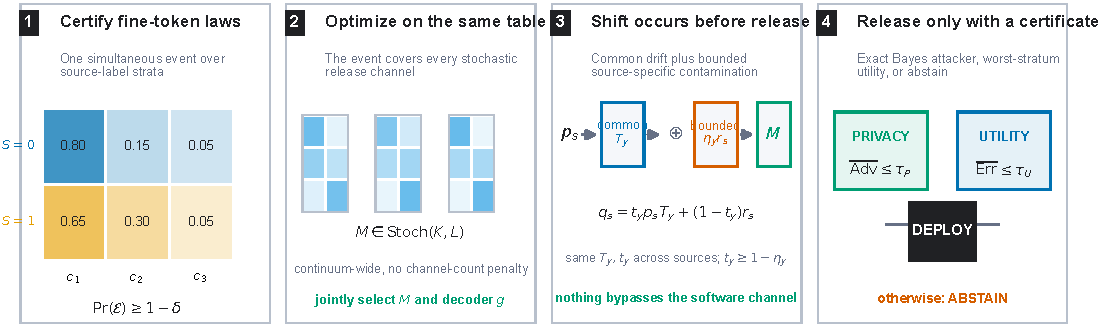
\includegraphics[width=\textwidth]{figures/figure1_mosaic_overview.pdf}
  \caption{MOSAIC certifies fine-token laws before applying a source-blind
  stochastic release. The same confidence event covers continuum channel and
  decoder selection. Structured shift acts before the enforced channel, and a
  release occurs only when both universal-attacker privacy and worst-stratum
  task utility pass; otherwise MOSAIC abstains.}
  \label{fig:overview}
\end{figure*}

\section{Related Work}

\paragraph{Erasure and universal representations.}
Linear and nonlinear concept-erasure methods remove directions, covariance, or
components associated with a source variable
\citep{ravfogel2020null,ravfogel2022linear,ravfogel2022kernel,
belrose2023leace,jourdan2023taco,holstege2025splince,
akbari2025obliviator,avitan2026mance}; causal interventions and leakage audits
also show why a weak probe is not a universal certificate
\citep{elazar2021amnesic,chowdhury2025limits,zarlenga2025leakage}. FARE
certifies every downstream classifier for a restricted finite representation,
while smooth-representation and adversarial-inference work develops other
finite-sample, high-confidence fairness guarantees
\citep{jovanovic2023fare,gitiaux2021smooth,deka2023mmdbfair,luo2025frg}.
MOSAIC differs narrowly: its confidence event is placed on pre-release token
laws, uniformly covering a stochastic post-channel optimized on that same
table and then transferred through an explicit shift class.

\paragraph{Randomized mappings and risk control.}
Probabilistic preprocessing, privacy funnels, and fair Pareto optimization
already establish that stochastic channels can improve population
privacy--utility tradeoffs
\citep{calmon2017preprocessing,makhdoumi2014privacyfunnel,
agarwal2024randomization,kozdoba2024pareto}. MOSAIC does not claim randomization
as new. Risk-controlling prediction, Learn-Then-Test (LTT), conformal risk
control, and Pareto testing certify registered decisions and abstain when none
passes \citep{bates2021rcps,angelopoulos2025ltt,angelopoulos2024crc,
laufer2023pareto,zollo2024prompt}. Robust conformal variants further address
specified covariate or likelihood-ratio shifts
\citep{tibshirani2019covariate,cauchois2024robust,almeida2025hprc,
zecchin2025wcrc}. These are the closest decision-layer precedents. MOSAIC's
distinct statistical object is one confidence region for a sufficient table:
it covers an uncountable channel family without testing channels separately or
paying a channel-count correction.

\paragraph{Shift, contraction, and abstention.}
Dobrushin coefficients quantify channel contraction and have been used for
privacy mechanisms and invariant domain generalization
\citep{diaz2018contractivity,shui2022regularization}. Fair-learning robustness
and impossibility results show that unrestricted shift precludes nontrivial
universal guarantees \citep{lechner2021impossibility,agarwal2025robustfair,
bendavid2010impossibility}. Benchmark and subgroup-robustness work documents
the corresponding empirical failures
\citep{koh2021wilds,sagawa2020groupdro,zhou2021spurious,
subbaswamy2021evaluation,hashimoto2018fairness,sohoni2020subclass,
kang2022certifying,ehyaei2025fragile}. We therefore state the common-transform
plus differential-contamination model explicitly and certify only conditionally
on membership in it. Explicit abstention follows selective-prediction practice
\citep{elyaniv2010foundations,geifman2017selective,geifman2019selectivenet,
timans2025monitoring}, but here it is triggered by a joint privacy--utility
release contract rather than predictive confidence alone.

\section{Problem Setup}

Let $S\in[G]$ denote source, $Y\in[J]$ task label, and $C\in[K]$ the fine token.
For a fixed label, write $p_s(c)=\Pr(C=c\mid S=s,Y=y)$. The source-blind release
channel $M$ produces $Z\in[L]$. The balanced accuracy of the strongest
downstream source attacker is
\begin{equation}
 A(P,M)=\frac{1}{G}\sum_{z=1}^{L}\max_{s\in[G]}(p_sM)(z),
 \label{eq:attacker}
\end{equation}
with normalized advantage
$\operatorname{Adv}_G(A)=(GA-1)/(G-1)$. This is chance-normalized and ranges
from zero to one.

For each supported source--label stratum, the certification table supplies an
empirical law $\widehat p_{s,y}$ and radius $\epsilon_{s,y}$. The simultaneous
event
\begin{equation}
 \mathcal E=\bigcap_{s,y}
 \{\|\widehat p_{s,y}-p_{s,y}\|_1\leq\epsilon_{s,y}\}
 \label{eq:event}
\end{equation}
has probability at least $1-\delta$ after a fixed allocation across strata. We
use the Weissman multinomial radius \citep{weissman2003l1} in the confirmation,
although any valid
simultaneous region can replace it. The tokenizer and fine alphabet must be
fixed without these observations.

The external law for label $y$ belongs to the structured class
\begin{equation}
 q_s=t_y p_sT_y+(1-t_y)r_s,
 \qquad t_y\geq 1-\eta_y,
 \label{eq:shift}
\end{equation}
where $T_y$ is a source-independent fine-token channel from a registered
convex uncertainty set and each residual $r_s$ is arbitrary. Both components
pass through the same release channel $M$. This placement is crucial: a
constant-row software channel cannot leak information that appears before it.

\section{Adaptive Universal-Attacker Certificate}

For a bounded vector $v$, define the exact confidence-set support function
\begin{equation}
 \Phi(\widehat p,\epsilon;v)=
 \max_{p\in\Delta_K:\|p-\widehat p\|_1\leq\epsilon}p^\top v.
 \label{eq:phi}
\end{equation}
It is obtained by moving at most $\epsilon/2$ mass from low to high
coordinates of $v$, or from an equivalent linear-program dual. For attacker
assignment $a\in[G]^L$, let
$v_{M,a,s}(c)=\sum_zM(c,z)\mathbf 1\{a(z)=s\}$. We then define
\begin{equation}
 \overline A(\widehat P,M)=\frac{1}{G}\max_{a\in[G]^L}
 \sum_s\Phi(\widehat p_s,\epsilon_s;v_{M,a,s}).
 \label{eq:abar}
\end{equation}

\begin{theorem}[Adaptive exact envelope]
On $\mathcal E$, simultaneously for every row-stochastic $M$, including a
channel selected as an arbitrary function of the same table,
$A(P,M)\leq\overline A(\widehat P,M)$. For fixed $M$, the right-hand side is the
exact supremum over the product of the stated $\ell_1$ confidence sets.
\end{theorem}

The proof writes the Bayes attacker as a maximum over deterministic assignments.
For a fixed assignment the source confidence sets separate, giving one support
function per source; all maxima are finite and commute. The implication is
pointwise over the complete stochastic-channel space, which is why adaptive
selection needs no channel-count correction.

\section{Certification under Pre-Release Shift}

Define the arbitrary differential-shift capacity
\begin{equation}
 \operatorname{Cap}_G(M)=\frac{1}{G}\max_{a\in[G]^L}
 \sum_s\max_c v_{M,a,s}(c).
 \label{eq:capacity}
\end{equation}
This equals $\sup_{r_1,\ldots,r_G}A(R,M)$. For $G=2$, its normalized value is
the Dobrushin coefficient, the largest total variation distance between two
rows of $M$.

For a transform polytope with registered extremes
$\mathcal V_y=\operatorname{ext}(\mathcal T_y)$, define the shifted envelope
\begin{equation}
 \begin{aligned}
 \overline A_y^X(M)
 &=\frac1G\max_{T\in\mathcal V_y,\,a\in[G]^L}\sum_s\Big[
 \\[-2pt]&\quad (1-\eta_y)
 \Phi(\widehat p_{s,y},\epsilon_{s,y};Tv_{M,a,s})
 \\[-2pt]&\quad +\eta_y\max_cv_{M,a,s}(c)\Big].
 \end{aligned}
 \label{eq:exactshift}
\end{equation}

\begin{theorem}[Transform-exact structured-shift certificate]
On $\mathcal E$, every same-table selected $M$ and every external law in
Eq.~\eqref{eq:shift} satisfy $A(Q,M)\leq\overline A_y^X(M)$. For fixed $M$,
the right-hand side is the exact supremum over the stated confidence sets,
transform polytope, retained masses, and arbitrary residual laws.
\end{theorem}

For fixed $T$, retained mass, and attacker assignment, the source confidence
sets and residual simplexes separate. Their support values are respectively
$\Phi(\widehat p,\epsilon;Tv)$ and $\max_cv(c)$. The latter is no smaller, so
the worst retained mass is $1-\eta_y$. The support objective is convex in $T$;
its maximum over a polytope occurs at an extreme. These finite maxima commute,
proving exactness. Since the statement holds pointwise for every $M$, it
survives adaptive channel selection.

When transform extremes cannot be enumerated, a capacity-transfer corollary is
available. Define
$\rho_T(M)=\max_c\operatorname{TV}((TM)(c,\cdot),M(c,\cdot))$ and
$B_y(M)=\min\{\operatorname{Cap}_G(M),
\overline A_y(\widehat P,M)+\rho_{\mathcal T_y}(M)\}$. Then
\begin{equation}
 A(Q,M)\leq(1-\eta_y)B_y(M)+\eta_y\operatorname{Cap}_G(M).
 \label{eq:transferbound}
\end{equation}
The exact envelope in Eq.~\eqref{eq:exactshift} is never larger. When
$\eta_y=0$ and $TM=M$, both reduce to the reference certificate; when
$\eta_y=1$, both reduce to exact distribution-free capacity.

\begin{proposition}[Exactness value]
For every $M$ and confidence table, the transform-exact privacy envelope is no
larger than Eq.~\eqref{eq:transferbound}. The matching transform-exact utility
value is likewise no larger than its capacity-transfer fallback.
\end{proposition}

Both exact quantities are suprema over the registered structured class. The
fallback proof upper-bounds every element of that same class using separate
contraction and capacity inequalities, so taking the supremum preserves the
ordering. The proposition holds pointwise in $M$; therefore optimizing the
tighter envelope cannot worsen the globally optimal certified objective. It can
still change feasibility sharply when a loose fallback straddles a contract
threshold, which is the effect tested in Fig.~\ref{fig:exactrefinement}.

For decoder $g:[L]\to[J]$, let
$u_y(c)=\sum_zM(c,z)\mathbf 1\{g(z)\neq y\}$. The matching exact conditional
error certificate is
\begin{equation}
 \begin{aligned}
 \overline E^X_{s,y}(M,g)
 &=\max_{T\in\mathcal V_y}\Big[
 (1-\eta_y)\\[-2pt]
 &\quad\Phi(\widehat p_{s,y},\epsilon_{s,y};Tu_y)
 +\eta_y\max_cu_y(c)\Big].
 \end{aligned}
 \label{eq:exactutility}
\end{equation}
It is the exact supremum over the same confidence and shift sets. Thus $M$,
$g$, privacy, and worst-stratum utility can all be selected on one event.

\begin{theorem}[No free lunch]
$\operatorname{Cap}_G(M)=1/G$ if and only if all rows of $M$ are identical.
For two sources, if two fine tokens carry different task labels and incur
row-wise decoder errors at most $e_0$ and $e_1$, then the normalized capacity is
at least $1-e_0-e_1$.
\end{theorem}

Consequently, unrestricted source-specific shift permits exact erasure only by
making the public token independent of the fine token. A bounded $\eta_y$ is
therefore an identifiable assumption of the deployment contract, not a hidden
technical convenience.

There is a separate identifiability boundary for external auditing. Suppose a
required source is absent and let
$A_{\rm miss}(q_0,M)=\sup_{q_1\in\Delta_K}A((q_0,q_1),M)$.

\begin{theorem}[Missing-source audit]
Any protocol with false-certification probability at most $\delta$ uniformly
over the unobserved law $q_1$ can claim
$A((q_0,q_1),M)\leq\tau<A_{\rm miss}(q_0,M)$ with probability at most
$\delta$.
\end{theorem}

The observed audit distribution is identical for every missing law; choosing a
simplex maximizer makes every stronger claim a false certification. The same
argument makes the utility bound for a missing source--label stratum at least
$\max_c(M\ell_y)(c)$. Missing required strata are therefore unestimable, not
evidence of safety; the supplement gives the full proof.

\section{Global Optimization and Abstention}

For fixed decoder, every support function in Eqs.~\eqref{eq:exactshift} and
\eqref{eq:exactutility}, transformed score, and residual row maximum has a
linear epigraph. Enforcing all registered transform extremes and all $G^L$
attacker assignments gives one linear program in the $KL$ channel entries.
Enumerating all $J^L$ decoders therefore yields the global finite-alphabet
optimum. The capacity-transfer fallback uses binary branch variables and one
mixed-integer linear program per decoder. A release is accepted only when the
solver reports optimality, all primal residuals pass, and separately recomputed
certificates agree with the objective; otherwise the rule abstains.

\paragraph{Release protocol.}
The end-to-end rule is deliberately mechanical. First, fix the tokenizer,
transform polytope, source and task alphabets, thresholds, and confidence
allocation without the certification fold. Second, form every supported
$\widehat p_{s,y}$ and simultaneous radius. Third, for each of the $J^L$
decoders, solve the exact LP minimizing worst certified utility subject to all
privacy constraints. Fourth, replay every certificate from the returned
channel and reject nonoptimal or numerically inconsistent solutions. Finally,
among any separately registered tokenizers or erasers, apply their familywise
allocation and select the feasible row with minimum certified error under a
fixed tie break. No feasible row, unsupported required stratum, or failed
solver check returns \textsc{abstain}; otherwise the software releases only
$(M,g)$ and the resulting token interface.

Let $R=\max_y|\mathcal V_y|$. For one decoder, a direct support-function
formulation has order
$KL+JR G^{L+1}K+JRGK$ variables and constraints: the middle term comes from
privacy transform--attacker--source tuples and the last from utility strata.
Thus the exact method is polynomial in the fine alphabet $K$ for fixed
$(G,J,L,R)$ but exponential in the deliberately small released alphabet $L$.
Decoder enumeration adds a factor $J^L$ and parallelizes exactly. Larger public
alphabets require separation or column-generation methods; the present theorem
does not hide that computational boundary.

The exact optimizer is checked against binary confidence-ball endpoint
enumeration, zero-radius population-risk identities, 100 randomized dominance
comparisons with the capacity-transfer bound, and dense stochastic-channel
grids. The fallback has separate randomized grid checks and a constructed
witness where stochastic release strictly beats every deterministic channel.
These checks validate the encodings but do not replace the algebra.

The locked analysis also predicts abstention as sample size changes. A
finite-sample envelope follows by enlarging population-centered confidence
balls: whenever the enlarged problem remains feasible, a Weissman union bound
controls the probability that the empirical optimizer abstains. Because this
bound can be loose near a decision boundary, we separately preregister a local
delta-method power curve. Under a unique stable branch and strong regularity of
the parametric linear program, centered simplex finite differences estimate the
value gradient and the stratified multinomial central limit theorem predicts
the deployment probability. A two-step gradient-stability check is required;
the approximation is rejected if it fails.

\section{Hash-Locked Evaluation}

\paragraph{Synthetic confirmation.}
The synthetic confirmation fixes two source--label populations, two structured
shift regimes, eight deployment rules, five possible per-stratum sample sizes,
and 1,000 independent tables per registered cell. Pilot seeds are permanently
excluded. Before confirmatory outcomes, the complete protocol, method code,
theorem text, evaluators, pilot history, pass criteria, and theory predictions
are SHA-256 locked and pushed to a public branch. Every selected channel is
graded by a separately implemented exact population evaluator that enumerates
common-transform extremes, attacker assignments, and residual simplex
vertices. The confirmation stores every channel, decoder, seed, decision,
confidence-event marker, and exact risk, then an independent script replays all
rows and aggregate intervals. This artifact-first protocol follows established
recommendations for model documentation, dataset documentation, internal
auditing, and reproducible ML reporting
\citep{mitchell2019modelcards,gebru2021datasheets,raji2020auditing,
pineau2021reproducibility}.

The hard-safety regime fixes contamination $\eta=0.20$, maximum source
advantage $\tau_P=0.30$, maximum worst-stratum error $\tau_U=0.40$, and
$n\in\{125,250,500\}$ observations per source--label stratum. The retention
regime uses $(\eta,\tau_P,\tau_U)=(0.10,0.35,0.45)$ and
$n\in\{125,250,500,1000,2000\}$. Both use familywise $\delta=0.05$, three
fine tokens, two released tokens, two registered common-transform extremes,
and 1,000 untouched tables per cell. The eight rules are always-deploy,
plug-in continuum selection, shift-unaware MOSAIC, held-out fixed-channel
certification, finite-grid LTT, deterministic MOSAIC, MOSAIC, and an
unattainable population oracle.

The primary safety contrast compares the plug-in continuum rule with MOSAIC at
a near-boundary shift contract. The primary usefulness contrast compares safe
retention against a held-out fixed-channel certificate, a finite-grid
Learn-Then-Test rule with simultaneous one-sided bounds, and deterministic
MOSAIC. The final gate additionally requires the preregistered theory curve to
track deployment across sample sizes. All methods and cells remain reportable
if any gate fails.

\section{Locked Synthetic Results}

All five preregistered gates passed. Here ``MOSAIC-transfer'' denotes the
capacity-transfer fallback used before the transform-exact refinement. The
independent replay recomputed 128,000
exact external risks and 128,000 deployment labels from 64,000 method-level
receipts with zero mismatch.  Figure~\ref{fig:confirmation} reports every
registered deployment rule in the two primary cells; the population oracle is
omitted from the bars because it is a feasibility diagnostic rather than an
implementable method.

\begin{figure*}[t]
  \centering
  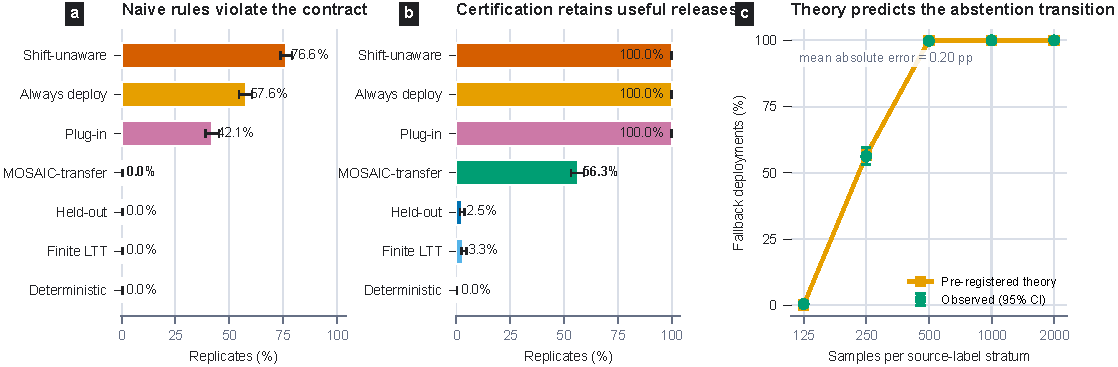
\includegraphics[width=\textwidth]{figures/figure2_mosaic_confirmation.pdf}
  \caption{Hash-locked confirmation with 1,000 independent certification
  tables per cell.  Error bars are exact 95\% Clopper--Pearson intervals.
  (a) At the hard safety boundary, plug-in continuum selection falsely accepts
  42.1\% of tables, whereas MOSAIC-transfer abstains and records no false acceptance.
  Ignoring registered shift is worse.  (b) In the feasible retention cell,
  MOSAIC-transfer safely deploys on 56.3\% of tables, compared with 2.5\% for a held-out
  fixed-channel certificate, 3.3\% for finite LTT, and 0\% for deterministic
  MOSAIC. Non-certifying rules happen to be safe in this easier cell but fail
  in panel (a).  (c) The deployment transition follows the theory curve frozen
  before outcomes (mean absolute error 0.20 percentage points).}
  \label{fig:confirmation}
\end{figure*}

\begin{table}[t]
\centering
\small
\setlength{\tabcolsep}{3.1pt}
\begin{tabular}{lrrr}
\hline
Rule & Deploy & False accept & Safe deploy \\
\hline
\multicolumn{4}{l}{\emph{Hard safety boundary, $n=125$}} \\
Always deploy        & 100.0 & 57.6 & 42.4 \\
Shift-unaware MOSAIC &  80.3 & 76.6 &  3.7 \\
Plug-in continuum    &  73.7 & 42.1 & 31.6 \\
\textbf{MOSAIC-transfer} & 0.0 & \textbf{0.0} & 0.0 \\
\hline
\multicolumn{4}{l}{\emph{Retention regime, $n=250$}} \\
Held-out fixed       &   2.5 &  0.0 &  2.5 \\
Finite LTT           &   3.3 &  0.0 &  3.3 \\
Deterministic MOSAIC &   0.0 &  0.0 &  0.0 \\
\textbf{MOSAIC-transfer} & \textbf{56.3} & 0.0 & \textbf{56.3} \\
\hline
\end{tabular}
\caption{Primary registered rates (\%).  Each row uses the same 1,000 tables
within a cell.  ``False accept'' means deployed while violating at least one
exact external privacy or utility contract.}
\label{tab:primary}
\end{table}

The safety contrast is paired: plug-in selection has 421 false acceptances
that MOSAIC-transfer avoids and there are no reverse discordances. The paired rate
difference is 42.1 points (bootstrap 95\% interval $[39.0,45.2]$; exact
McNemar $p=3.69\times10^{-127}$). Across all eight registered fallback cells,
including 8,000 independently sampled certification tables, no accepted
release violates the exact external contract.  This is finite-run evidence
consistent with the theorem, not a replacement for its $1-\delta$ guarantee.

In the retention cell, MOSAIC-transfer improves safe deployment over held-out
certification by 53.8 points ($[50.6,56.9]$), finite LTT by 53.0 points
($[49.9,56.1]$), and deterministic MOSAIC by 56.3 points ($[53.2,59.3]$);
all paired exact $p$-values are below $2.1\times10^{-158}$.  The stochastic
comparison is essential: no deterministic channel satisfies the same
finite-sample contract in this cell. Fallback deployment rises from 0.5\% at
$n=125$ to 56.3\% at $n=250$, 99.8\% at $n=500$, and 100\% at $n\geq1000$.
The preregistered local power approximation has 0.20-point mean absolute error
over these five sizes and 0.44-point error at the primary size.  Its active-set
and two-step gradient-stability diagnostics pass at every registered point.


\input{mosaic_transform_exact_results}

\paragraph{Official-method real-feature confirmation.}
A separate pre-outcome lock evaluates five frozen feature stores spanning
vision (Waterbirds), medical vision (Camelyon17-WILDS), text
(CivilComments-WILDS and BiasBios), and gait time series
\citep{sagawa2020groupdro,koh2021wilds,borkan2019civilcomments,
dearteaga2019bios,goldberger2000physionet}. For every dataset and each untouched seed in
$\{100,\ldots,104\}$, the construction split fits a balanced logistic task
score and discretizes it at quartiles into four fine tokens. MOSAIC releases
two tokens under identity or registered 10\% adjacent-token smoothing, with
$(\eta,\tau_P,\tau_U,\delta)=(0.05,0.35,0.49,0.05)$.
This pre-refinement lock uses the capacity-transfer fallback; the paired
synthetic amendment isolates the exact-envelope gain.

The frontier contains identity and twelve settings from the pinned official
INLP, LEACE, R-LACE, TaCo, and MANCE++ implementations
\citep{ravfogel2020null,belrose2023leace,ravfogel2022linear,
jourdan2023taco,avitan2026mance}. Each edit has its own tokenizer, so the
familywise event allocates $\delta/13$ per candidate; continuum channel
selection within each fixed table incurs no additional correction. Among
candidates that pass both certificates, the rule selects minimum certified
worst-stratum error with a lexical tie break. Every receipt stores the complete
token tables, channel, decoder, solver checks, decision, and natural external
diagnostic. An independent program reconstructs every radius, certificate,
selection, and diagnostic. External splits test empirical behavior but do not
establish membership in Eq.~\eqref{eq:shift}; missing source--label strata are
reported as unestimable rather than safe.

\section{Official-Method Feature Results}

All 25 dataset--seed jobs and all 325 registered candidate rows completed with
no proxy implementations or optimization failures. The independent replay
reconstructed every confidence radius, certificate, selected channel, decoder,
external diagnostic, and lexical tie break with zero mismatch. Table
\ref{tab:realfrontier} reports the complete selection behavior.

\begin{table*}[t]
\centering
\small
\setlength{\tabcolsep}{5.1pt}
\begin{tabular}{llclcl}
\hline
Dataset & Modality & Deploy & Selected family & Best cert. error & Natural external diagnostic \\
\hline
Waterbirds & vision & 0/5 & -- & .499 & 1/65 candidate rows safe; none certified \\
Camelyon17-WILDS & medical vision & 5/5 & LEACE (5) & .282 & unestimable: required source absent \\
CivilComments-WILDS & text & 0/5 & -- & .500 & 0/65 candidate rows safe \\
BiasBios-Clinical & clinical text & 5/5 & INLP (4), R-LACE (1) & .312 & 5/5 selections safe; 65/65 rows safe \\
GaitPDB & time series & 0/5 & -- & .500 & 0/65 candidate rows safe \\
\hline
\end{tabular}
\caption{Locked official-method frontier, five seeds per dataset and 13
candidates per seed. ``Best cert. error'' is the mean selected value for
deployment rows and the mean minimum available value for abstention rows.
External diagnostics are descriptive and do not establish structured-shift
membership.}
\label{tab:realfrontier}
\end{table*}

BiasBios provides the positive real-feature case. Every official candidate
clears both contracts on all five seeds; MOSAIC selects INLP four times and
R-LACE once. The selected mean certified worst error is .312 (range
.299--.326), while the natural external diagnostic has mean worst error .194
and mean source advantage .061. All five estimable selections are externally
safe, although five seeds are too few for a strong frequency claim.

An audited post-outcome exact replay improves 133 of 325 objectives and adds two
diagnostically safe Waterbirds deployments; it is exploratory and does not
establish shift-class membership.

The negative rows explain why an explicit release rule matters. Every candidate
in Waterbirds, CivilComments, and GaitPDB clears the privacy threshold only by
giving a certified worst error near .50, above the registered .49 utility
contract, so MOSAIC abstains on all 15 jobs. Natural external diagnostics agree
on CivilComments and GaitPDB; one of 65 Waterbirds candidates happens to be safe
externally but is not certifiable from its construction table. Conversely,
Camelyon17 produces five certifiable LEACE releases under the registered shift
model, but its natural external split lacks a required source class. The
missing-source theorem therefore forces the external result to be labeled
unestimable. Across the five externally estimable selected releases there are
zero false acceptances; this is a diagnostic check, not proof that the benchmark
splits satisfy Eq.~\eqref{eq:shift}.


\section{Guarantee Semantics}

\paragraph{Probability and deployment shift.}
The probability $1-\delta$ is over the certification table. On its simultaneous
event, the conclusion holds uniformly over every optimized channel and every
external distribution in the registered shift class. It does not assume that
an external metric is within a validation confidence interval. Instead,
$(\mathcal T_y,\eta_y)$ are explicit contract parameters: common transformations
inside $\mathcal T_y$ and up to $\eta_y$ arbitrary differential contamination
are already inside the external supremum. A natural benchmark split can reveal
a contradiction or missing support, but a favorable score cannot establish
membership in that class.

\paragraph{Where multiplicity is paid.}
The tokenizer is frozen before certification, and one confidence event on its
fine-token table covers the uncountable set of stochastic $M$ and every decoder
selected afterward. There is therefore no channel-count correction. If the
frontier contains $m$ separately learned erasers or tokenizers, their $m$
different tables do require a registered familywise allocation, as in the
official-method study. This is the precise distinction from applying LTT to a
finite list of already constructed channels: MOSAIC pays for statistical
objects, not for every point subsequently optimized inside one covered object.

\paragraph{Threat surface.}
The attacker knows $M$ and may use any function of the released token $Z$;
Eq.~\eqref{eq:attacker} is its exact balanced Bayes success, with no probe or
computational restriction. The guarantee requires $M$ to be source-blind and
software-enforced and $Z$ to be the only public representation interface.
Releasing $C$, the original feature vector, source-dependent metadata, or a
side channel falls outside the theorem. The task decoder may be public because
utility is certified jointly rather than treated as secret.

\section{Limitations and Scope}

The guarantee is conditional on Eq.~\eqref{eq:shift}; an ordinary benchmark
split cannot prove that a real hospital, text domain, or sensor environment
belongs to that class. Membership requires an engineering specification or
separate bridge data containing every required source--label stratum, with its
own confidence allocation. Without that evidence, a favorable score cannot
establish membership. The finite-token theorem also fixes the tokenizer and
alphabet independently of the certification table; large alphabets may require
structured confidence regions or column generation.

MOSAIC certifies source inference from the released token, not every possible
harm associated with representation use. It does not protect information that
is released through a separate interface, and it cannot recover utility that
the privacy contract makes information-theoretically impossible. Finally, the
novelty claim concerns the complete adaptive and shift-aware construction; its
classical ingredients must remain attributed to their respective literatures.

\section{Conclusion}

MOSAIC treats representation editing as release-mechanism design rather than a
probe contest. By certifying fine-token laws before a stochastic post-channel,
it can optimize over a continuum on the same table while retaining a single
finite-sample event. The structured shift theorem separates common drift that
the channel can absorb from differential drift that its capacity must pay for,
and the no-free-lunch result states when abstention is unavoidable. The locked
evaluation shows both sides of that decision: abstention at an infeasible safety
boundary and substantially higher safe retention when exact shift geometry can
replace a generic capacity bound.
